\documentclass[preprint]{aastex} 

\usepackage[top=1in, bottom=1in, left=1in, right=1in]{geometry}
\usepackage{amsmath}
\usepackage{graphicx}
\usepackage{mdwlist}
\usepackage{natbib}
\usepackage{natbibspacing}
\setlength{\bibspacing}{0pt}
\setlength{\parskip}{0pt}
\setlength{\parsep}{0pt}
\setlength{\headsep}{0pt}  
\setlength{\topskip}{0pt}
\setlength{\topmargin}{0pt}
\setlength{\topsep}{0pt}
\setlength{\partopsep}{0pt}
\setlength{\footnotesep}{8pt}
\pagestyle{empty}
\citestyle{aa}

\newcommand{\simgt}{\stackrel{>}{_{\sim}}}
\def\kperp{k_{\bot}}
\def\kpar{k_{\|}}
\def\k{{\bf k}}
\def\sky{{\theta}}
\def\HI{{H{\small I }}}
\def\HII{{H{\small II }}}
\def\xHI{{x_{\rm\HI}}}

\def\EnumCompress{\parskip-4pt}

%\usepackage{subfig}
%\usepackage[countmax]{subfloat}

\begin{document}
\title{Data Management Plan}

% Plans for data management and sharing of the products of research. Proposals must include a supplementary document of no more than two pages labeled “Data Management Plan”. This supplement should describe how the proposal will conform to NSF policy on the dissemination and sharing of research results (see AAG Chapter VI.D.4), and may include:
% 
%     the types of data, samples, physical collections, software, curriculum materials, and other materials to be produced in the course of the project;
% 
%     the standards to be used for data and metadata format and content (where existing standards are absent or deemed inadequate, this should be documented along with any proposed solutions or remedies);

% 
%     policies for access and sharing including provisions for appropriate protection of privacy, confidentiality, security, intellectual property, or other rights or requirements;
% 
%     policies and provisions for re-use, re-distribution, and the production of derivatives; and
%

%(see \S\ref{sec:DataProducts}).  

%     plans for archiving data, samples, and other research products, and for preservation of access to them.


This proposal will involve the collection and analysis data from the HERA-331 instrument, as well as its design and construction.  An overview is given in Figure \ref{fig:dmpBlock}.

We distinguish three distinct locations where data are processed and stored: the Karoo Array Processing Building ({\bf KAPB}) in South Africa, at the University of Pennsylvania ({\bf Penn}) and at the Massachusetts Institute of Technology ({\bf MIT}).  The KAPB serves as the storage point for the rawest form of the data.  The primary data archive for subsequent analysis is at Penn;  data internal to the collaboration will be distributed from this server via account access.  All publicly available data will be available via the Internet from the MIT server. 

\begin{figure}[h]
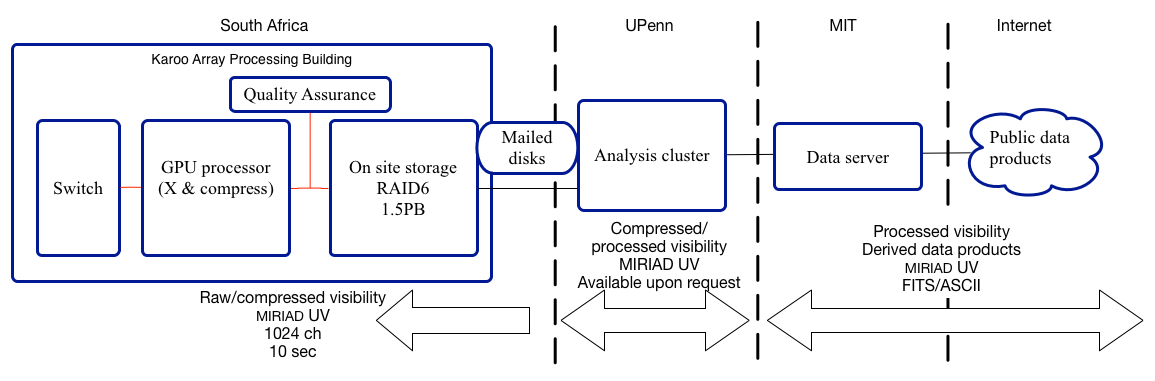
\includegraphics[width=\textwidth]{plots/Engineering/dataMgmtBlock.png}
\caption{Block diagram of HERA data system.  The dashed vertical lines denote different physical locations and the big arrows denote data regimes.}
\label{fig:dmpBlock}
\end{figure}

\section{Data Types}

Briefly, the data path is as follows. Raw data generated by the HERA correlator is transferred to a RAID system in the KAPB, and compressed on-site using the correlator X-Engines running during the day.  Real-time calibration is performed on data using the Quality Assurance (QA) cluster in the KAPB.  The QA cluster also generates a searchable observation database and metadata related to the array performance and data quality.
Compressed data is stored on-site, and is also transferred to Penn via streaming over the Internet, as well as being transferred to small disks which are mailed.  Further data analysis and reduction, including refined calibration and time-averaging over repeated observations, are performed on the Penn cluster.  Initially, this will use co-PI Aguirre's cluster and network storage (see Facilities, Equipment, and Other Resources), but will eventually be augmented to a 30-node dedicated cluster plus 250 TB storage for full HERA-331 operation. Subsets of the data in various forms are distributed to collaborators for further analysis.  Further data products include images, source catalogs, and models of diffuse emission.  

Below we specifically indicate the types of data generated, their format and content, the policies for distribution and archiving of each data type.

\noindent {\bf Raw visibility data.}  This is the raw output of the correlator, which is generated for each baseline at a cadence of approximately 10 seconds, with 1024 spectral channels.  This dataset is stored in the interferometric standard {\sc miriad}-UV files.  It is archived in the KAPB indefinitely using RAID6 storage devices.  Because of its large size, no plan is made for public distribution, though requests for this higher cadence data from interested scientists will be honored on a best-effort basis.
 
\noindent {\bf Compressed visibility data.}  This data has been reduced by a factor of $\sim$20 over the raw data, as described in the Project Description.  This data forms the core of the analysis effort by the collaboration and is stored in both the KAPB and at Penn.  It is served to collaborators from the Penn server.  The format is {\sc miriad}-UV files.
 
\noindent {\bf Calibration and observing Database and metadata.}  This will be made available to collaborators through the Penn and KAPB servers as necessary for observation management and subsequent data analysis.  The database will be in standard SQL form.
 
\noindent {\bf Compressed, time-averaged, and calibrated visibility data.}  {\it We are committing to publicly releasing this 18 months after data acquisition has ceased, for each season of observation.}      
Thus, according to the nominal timeline in the Project Description, the first observing season would end in mid-2015, and this data release would then occur in January 2017, with a similar schedule thereafter.  This schedule is of course subject to the revision based on the actual observing.  The data to be released has been averaged in time over redundant observations to reduce data volume, and represents the rawest form of data made available as a matter of course.  It is expected that this form of the data will be sufficient for re-analysis of our derived results or detailed comparison against other data sets.  The calibration will be the best available at the time of release, and the data will be accompanied with sufficient information on the observing details so that users can make quality assessments.  The format is again {\sc miriad}-UV files.   This data will be available over the Internet from the MIT server.  Resources exist to maintain the archive beyond the grant to honor the  public release of data after the 18-month proprietary period.
 
\noindent {\bf Derived Data Products.}  These include images of both foregrounds and high-redshift HI emission, source catalogs, and models of diffuse foreground emission.  Imaging products will include coarse real-time calibrated snapshot images as well as high dynamic range survey maps from the FHD pipeline.  Source catalogs will be derived, and a Global Sky Model of diffuse foregrounds will be updated with new observations and released.  These products will be available on the public server at MIT, and will be provided as they are generated and quality-assessed.  Finally, foreground-subtracted data cubes of high-redshift $21\,\textrm{cm}$ intensity maps and the associated ionization field will be available for cross-correlation studies, as well as to provide context for high redshift optical and IR studies.  These are only expected to be available after the HERA-331 observing season.  Maps will be in FITS format, and catalogs will be made available in FITS or ASCII format, and published to be compatible with Vizier (see e.g., Jacobs et al 2011 and Williams et al 2011).  

\noindent {\bf Software.}  Data reduction will use 1) internally generated custom software, 2) the open-source AIPY\footnote{\tt https://pypi.python.org/pypi/aipy} package, 3) publicly available packages (e.g. CASA\footnote{ \tt http://casa.nrao.edu/} and {\sc miriad}).  The data reduction will be described by publication in refereed articles.  

% Final antenna element construction schematics will be made available for future production of the HERA elements. These designs will be in industry standard format. Data collected about the electromagnetic properties of the small array will be disseminated in a scientific publication characterizing in detail the
% performance of the HERA elements.

 
% The calibration, imaging, and data-reduction pipelines associated with
% evaluating the performance of the 7-element hexagonal close-packed array
% will be
% implemented using the open-source AIPY software framework, and will run on the
% computing cluster and data archive for PAPER
% that is maintained at UPenn.  This currently consists of 22 nodes connected by Gb
% ethernet. These nodes consist of 16 Dell PowerEdge 1950s (dual 4-core Intel Xeon L5420 \@ 2.50GHz)
% and 6 Dell PowerEdge R410 (32 GB RAM; dual 6-core Intel Xeon E5649 \@ 2.53GHz),
% for a total of 200 cores and 448 GB RAM.  Fast working data storage is provided
% by a network storage system (NSS) based around two Dell MD1200s, with a total
% RAID storage capacity of 140 TB.

\end{document}
